% This file is part of Oaklisp.
%
% This program is free software; you can redistribute it and/or modify
% it under the terms of the GNU General Public License as published by
% the Free Software Foundation; either version 2 of the License, or
% (at your option) any later version.
%
% This program is distributed in the hope that it will be useful,
% but WITHOUT ANY WARRANTY; without even the implied warranty of
% MERCHANTABILITY or FITNESS FOR A PARTICULAR PURPOSE.  See the
% GNU General Public License for more details.
%
% The GNU GPL is available at http://www.gnu.org/licenses/gpl.html
% or from the Free Software Foundation, 59 Temple Place - Suite 330,
% Boston, MA 02111-1307, USA


\chapter{Numbers} \label{numbers}

\index{\texttt{number}} \index{\texttt{real}} \index{\texttt{complex}}
\index{\texttt{rational}} \index{\texttt{float}} \index{\texttt{integer}}
\index{\texttt{fraction}} \index{\texttt{fixnum}} \index{\texttt{bignum}}

\begin{figure}[h]
\centering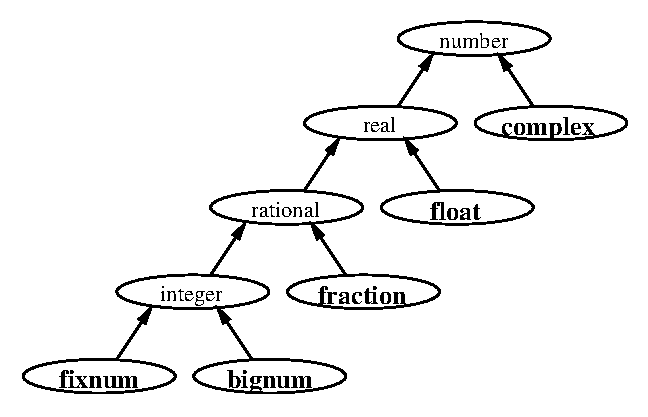
\includegraphics{numhier}
\caption{The numeric type hierarchy.  Abstract types are in plain face
and instantiable ones in bold.  Floating point numbers are not
implemented.} \label{fig:numhier}
\end{figure}

\section{Arithmetic}

\op{+}{\dt numbers}
\op{1+}{n}
\op{-}{n1 n2 \dt numbers}
\op{-}{n}
\op{*}{\dt numbers}
\op{/}{n1 n2}
\op{quotient}{n1 n2}
\op{modulo}{n1 n2}
\op{abs}{n1}
\op{max}{n1 n2}
\op{min}{n1 n2}
\op{expt}{n1 n2}


\section{Comparison}

\op{=}{n1 n2}
\op{{\protect\bang}=}{n1 n2}
\op{<}{n1 n2}
\op{>}{n1 n2}
\op{<=}{n1 n2}
\op{>=}{n1 n2}


\section{Predicates}

\pr{zero?}{n}
\pr{negative?}{n}
\pr{positive?}{n}
\pr{even?}{n}
\pr{odd?}{n}
\pr{factor?}{n1 n2}


\section{Rounding}

These operations should work on any subtype of \df{real}.

\op{floor}{x}
\doc{Returns the largest integer less than or equal to \emph{x}.}

\op{ceiling}{x}
\doc{Returns the smallest integer greater than or equal to \emph{x}.}

\op{truncate}{x}
\doc{Could be defined \texttt{(if (negative?\ x) (ceiling x) (floor x))}.}

\op{round}{x}
\doc{Returns nearest integer to \emph{x}.  Ties are broken by rounding
to an even number.}

\section{Bitwise Logical Operations}

These operations are only defined for integers.

\op{ash-left}{i amount}
\op{ash-right}{i amount}
\op{rot-left}{i amount}
\op{rot-right}{i amount}
\op{bit-not}{i}
\op{bit-and}{i1 i2}
\op{bit-or}{i1 i2}
\op{bit-nor}{i1 i2}
\op{bit-xor}{i1 i2}
\op{bit-nand}{i1 i2}
\op{bit-andca}{i1 i2}
\op{bit-equiv}{i1 i2}


\section{Accessing Components}

\op{numerator}{rational}
\op{denominator}{rational}

\op{real-part}{number}
\op{imag-part}{number}
